% !TeX root = paper.tex


\chapter{システム概要}
\section{この章で書くこと}
\begin{itemize}
	\item 識別,分類とは
	\item 現存するサービスでできること
	\item 概要図
	\item モデルについて
	\item サーバ関連について
	%\item もしかしたらあんまり書くことないかも
\end{itemize}
\section{識別,分類とは}
識別とは,・・・・・・\\
分類とは,・・・・・・
\section{現存するサービス}
\begin{itemize}
	\item Google レンズ
	\item YOLO
\end{itemize}

\subsection{Googleレンズ}\label{google-service}
これは画像の分類を行うアプリである.単に分類結果が表示されるのではなく,分類したいオブジェクトが映っているウェブサイト一覧が表示されるものである.表示されたウェブサイトを適当に選び自分が知りたい結果をウェブサイトの中から探し出す必要がある.また,一枚の画像に複数のオブジェクトが存在している場合は正しい結果が得られない.

\subsection{YOLO}\label{YOLO-service}
YOLOの説明いいいいい

YOLOでは,学習データを準備し学習させることで任意のオブジェクトを判別できるモデルの開発ができる.
本プロジェクトでは,YOLOを用いて電車の車両タイプを識別,分類する2つのモデルを開発する.
\section{システム概要図}
本プロジェクトで開発するシステム概要を図\ref{FIG}に示す.システムは車両判別部とUIに分けられる.\\
\red{田村と相談,画像は後で変える}

\begin{figure}
	\centering
	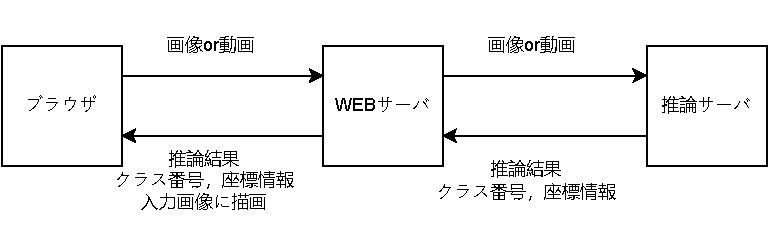
\includegraphics [width=\linewidth]{fig/system.pdf}
	\caption{システム概要図}
	\label{FIG}
\end{figure}






